\documentclass[reprint, aps, prx, amsmath, amssymb, longbibliography, superscriptaddress]{revtex4-2}

%% don't need amsmath because it is loaded in \documentclass
%% \usepackage{amsmath,amssymb}
\usepackage{graphicx}
\usepackage{epsfig}
\usepackage{mathrsfs,esint}
\usepackage{physics}
\usepackage{relsize}
\usepackage{bbold}
%% \usepackage{float} %% revtex4-2 has a conflict with float
\usepackage{dsfont}
\usepackage{comment}
\usepackage{svg}
\usepackage{enumitem}

%% packages for combining several images into a single figure
%%\usepackage{caption}
%%\usepackage{subcaption}
\usepackage[caption=false]{subfig}

%% Hyperref loaded the last because some packages may redefine \label
\usepackage[bookmarks=true,
   colorlinks=true,
   linkcolor=blue,
   urlcolor=blue,
   citecolor=blue,
   bookmarks=true,
   hyperindex=true
]{hyperref}
%\usepackage{natbib}

% todo package
\usepackage{todonotes}

\definecolor{mediumtealblue}{rgb}{0.0, 0.33, 0.71}
\newcommand{\jk}[1]{{\color{mediumtealblue}#1}}
\newcommand{\al}[1]{{\color{purple}#1}}
\newcommand{\dl}[1]{{\color{red}#1}}
\newcommand{\dk}[1]{{\color{blue}#1}}
\newcommand{\vk}[1]{{\color{green}#1}}

\DeclareMathOperator{\Zn}{\mathbb{Z}_n}
\DeclareMathOperator{\Zthree}{\mathbb{Z}_3}
\DeclareMathOperator{\Ztwo}{\mathbb{Z}_2}
\DeclareMathOperator{\Id}{Id}
\DeclareMathOperator{\diag}{diag}
\DeclareMathOperator{\sgn}{sign}


\begin{document}

\title{From \texorpdfstring{$\Zthree$}{Z3} Rabi model to Potts model}

\author{Anatoliy I. Lotkov}
\affiliation{Department of Physics, University of Basel, Klingelbergstrasse 81, CH-4056 Basel, Switzerland}

\author{Valerii K. Kozin}
\affiliation{Department of Physics, University of Basel, Klingelbergstrasse 81, CH-4056 Basel, Switzerland}


\author{Denis V. Kurlov}
\affiliation{Department of Physics, University of Basel, Klingelbergstrasse 81, CH-4056 Basel, Switzerland}


\author{Jelena Klinovaja}
\affiliation{Department of Physics, University of Basel, Klingelbergstrasse 81, CH-4056 Basel, Switzerland}

\author{Daniel Loss}
\affiliation{Department of Physics, University of Basel, Klingelbergstrasse 81, CH-4056 Basel, Switzerland}

%%%%%%%%%%%%%%


\begin{abstract}
% We study one- and two-mode variants of the $\Zthree$ Rabi model, investigate their spectral properties. For the two-mode $\Zthree$ Rabi model we derive a mapping onto a qubit-boson ring.

In this paper we study the $\Zthree$-symmetric Rabi models that describe a three-level system coupled to one or more boson modes. In particular, we focus on the models with one and two boson modes and determine their spectra. Next, we derive a mapping of the two-mode $\Zthree$ Rabi model onto a qubit-boson ring. This mapping allows us to formulate a realistic implementation of the $\Zthree$ Rabi model based on superconducting qubits. It also provides a context for the previously proposed optomechanical implementation of the $\Zthree$ Rabi model. In addition, we propose a physical implementation of the $\Zthree$ Potts model via a coupled chain of $\Zthree$ Rabi models.
\end{abstract}

\maketitle


\section{Introduction}

The field of quantum simulations has entered a mature phase in which a variety of hardware platforms can reproduce many-body Hamiltonians that are analytically intractable. Trapped-ion chains have been used to implement long-range Ising model and lattice gauge theories with tens of qubits \cite{tan_domainwall_2021, kyprianidis_observation_2021,brydges_probing_2019,zhang_observation_2017,martinez_realtime_2016,meth_simulating_2025}; neutral-atom Rydberg arrays routinely emulate spin models on two-dimensional lattices \cite{madjarov_highfidelity_2020,semeghini_probing_2021,scholl_quantum_2021,manovitz_quantum_2025,bernien_probing_2017}; and semiconductor spin-qubit platforms have realized Fermi–Hubbard and other models at the few-plaquette level \cite{dehollain_nagaoka_2020, hensgens_quantum_2017, kiczynski_engineering_2022, vandiepen_quantum_2021, wang_experimental_2022, wang_probing_2023}. These successes show that controlled, programmable devices can already access a wide variety of interesting physics such as symmetry breaking, topological order, and non-equilibrium critical phenomena that lie well beyond classical reach. One of the interesting research directions is to simulate models with larger discrete symmetries, e.g., $\Zthree$ symmetry, as they often exhibit richer physics than the models with the $\Ztwo$ symmetry.
% and to explore whether the associated phase transitions remain continuous or become first-order

Recent advances in circuit quantum electrodynamics (cQED) provide a complementary route to this goal, focusing on light–matter systems where photons mediate interactions between superconducting qubits~\cite{kurpiers_deterministic_2018,vanloo_photonmediated_2013,astafiev_resonance_2010}. In cQED, the quantum Rabi model \cite{braumuller_analog_2017, braak_integrability_2011,hwang_quantum_2015, chen_shortcuts_2021} --- describing a two-level atom coupled to a boson mode --- serves as the canonical building block and possesses a discrete $\Ztwo $ (parity) symmetry. At the ultrastrong coupling regime, a chain of coupled Rabi models effectively realizes the Ising model~\cite{hwang_largescale_2013}. There, photon-induced interactions generate nearly degenerate “cat” ground states with macroscopic qubit–cavity entanglement. Extending this connection between discrete symmetries and entangled phases from $\Ztwo$ to $\Zthree$ \cite{albert_quantum_2012, zhang_z_n_2014, sedov_chiral_2020, kozin_quantum_2024} naturally leads to the paradigmatic three-state Potts model and promises richer symmetry-breaking behavior.
Recently, there has been a significant interest in the $\Zthree$ quantum Rabi model from both theoretical and experimental perspectives. 
The generalization of Albert et al. of the original ($\Ztwo$) Rabi Hamiltonian to an $N$-state atom  \cite{albert_quantum_2012} established the formal framework to study the gneralized Rabi models with higher discrete symmetries. Subsequently, the first proposal for experimental realization of the $\Zthree$ Rabi model based on the optomechanical system was discussed in Ref.~\cite{sedov_chiral_2020}. Interestingly, it was shown that in the $\Zthree$ Rabi model the superradiant transition is first-order within the mean-field approach, unlike in the $\Ztwo$ Rabi model, where it is second-order~\cite{sedov_chiral_2020}. A recent proposal have shown how a network of Josephson junctions can implement the $\Zthree$ Potts model using tunable inductive elements \cite{wauters_engineering_2024}. Here we introduce a tunable model that connects the $\Zthree$ Rabi with the $\Zthree$ Potts model. By varying the coupling parameter, the system evolves from a few-level regime into one that spontaneously breaks the threefold rotational symmetry. 

The rest of the paper is organized as follows. In Sec.~\ref{sec:z3-rabi}, we give a brief overview of the $\Zthree$ Rabi model, derive the mapping of the $\Zthree$ Rabi model onto a certain qubit-boson model. We then illustrate how this qubit-boson model can be realized by superconducting-qubit and optomechanical platforms. In Sec.~\ref{sec:potts-model}, we show how the $\Zthree$ Potts model can be simulated by a chain of the $\Zthree$ Rabi models. We also illustrate it with the superconducting and optomechanical implementations. At the end of Sec.~\ref{sec:potts-model}, we briefly discuss the chiral $\Zthree$ Potts model and the possibility of its implementation based on a chain of the $\Zthree$ Rabi models. Finally, in Sec.~\ref{sec:conclusion}, we conclude. Some additional details are covered in Apps.~\ref{app:arbitrary-interaction-summary}-\ref{app:disorder}.



\section{\texorpdfstring{$\Zthree$}{Z\_3} Rabi model.}
\label{sec:z3-rabi}

\subsection{Theoretical description}
\label{sec:rabi-theory}

The central theme of this paper is the $\Zthree$-symmetric Rabi and Potts model as well as the connection between them. In this section, we give a brief description of the $\Zthree$ Rabi model. For the more detailed discussion, we refer the reader to our companion paper \cite{lotkov_cat_2025b}. In particular, we talk about the two-mode variation of the $\Zthree$ Rabi model because it maps onto the qubit-boson ring (see Sec.~\ref{sec:physical-implementation}). It describes the $\Zthree$-symmetric interaction of two boson modes and a three-level system, qutrit. The model's Hamiltonian is
\begin{equation}
\label{eq:2-mode-z3-Rabi}
\begin{aligned}
     H_{\text{R}} = &\hbar \Omega_{\text{R}} (\hat a_1^{\dagger} \hat a_1 + \hat a_2^{\dagger} \hat a_2) + B (e^{i\phi} Z + e^{-i\phi} Z^{\dagger}) \\
    &- \lambda (\hat a_1 + \hat a_2^{\dagger}) X - \lambda (\hat a_1^{\dagger} + \hat a_2) X^{\dagger},
\end{aligned}
\end{equation}
where $\hat a_i^{\dagger}\  (\hat a_i)$ with $i = 1,2$ are boson creation (annihilation) operators \footnote{Note that we use hats to distinguish the boson operators, $\hat a,\, \hat a^{\dagger},\, \hat x, \,\hat p$.}, $X$ and $Z$ are $3\times 3 $ matrices generalizing the Pauli matrices (usually referred to as the shift and clock matrices, respectively). have the following physical meaning: $\Omega_{\text{R}}$ is the frequency of the two boson mode, $B$ and $\phi$ define the qutrit energy levels, $\lambda$ is the coupling strength between the boson modes and the qutrit, $\hbar$ is the Planck constant.

The $\Zthree$ shift $X$ and clock $Z$ matrices are a standard tool for describing the qutrit systems. They are defined by
\begin{equation}
\label{eq:shift-clock-matreces}
    X = \begin{pmatrix} 
         0 & 0 & 1 \\
         1 & 0 & 0 \\
         0 & 1 & 0 
        \end{pmatrix}, \quad
    Z = \begin{pmatrix}
         1 & 0 & 0 \\
         0 & \omega & 0 \\
         0 & 0 & \omega^2
        \end{pmatrix},
      \end{equation}
where $\omega = \exp[2\pi i/3]$ is the principle cubic root of unity. The clock and shift matrices are unitary, $ X X^{\dagger} = \mathbb{1}, \, Z Z^{\dagger} = \mathbb{1}$, but not Hermitian, $ X^{\dagger} \neq X, \, Z^{\dagger} \neq Z$. Therefore, the analogy between them and the Pauli matrices is not full. But the $X$ and $Z$ matrices allow us to generalize the qubit Pauli group $\mathrm{G}_2 = \langle \pm i^j \omega_z^k \omega_x^l\rangle_{j,k,l = 0}^1$ to the qutrit Pauli group $\mathrm{G}_3 = \langle \pm \omega^j Z^k X^l\rangle_{j,k,l= 0}^{2}$ \cite{gottesman_faulttolerant_1999}. The elements of the group $\mathcal{P}_3$ generate a basis for the qutrit operators.

The $\Zthree$ symmetry group for the qutrit appears naturally as a part of the qutrit Pauli group $\mathcal{P}_3$. Actually, there are two $\Zthree$ subgroups in the $\mathcal{P}_3$ group: generated by the powers of the matrix $X$ and $Z$. While both subgroups are conjugate to each other, here we choose the subgroup generated by the $Z$ matrix, $\Zthree = \langle Z^k \rangle_{k=0}^2$. The boson part of the $\Zthree$ symmetry is simply a residue of the bosonic $\mathrm{U(1)}$ symmetry. As a result, the $\Zthree$ symmetry generator has the following form:
\begin{equation}
     \mathcal{P}_{\text{R}} = \exp\left[\frac{2\pi i}{3}(\hat a_1^{\dagger}  \hat a_1 -  \hat a_2^{\dagger}  \hat a_2)\right] Z.
\end{equation}
As a consequence of the symmetry, the number of the first boson excitations minus the number of the second boson excitations and plus the number of the qutrit excitations is conserved modulo 3. While this requirement is not particularly straightforward, it is necessary for the rest of our arguments to work. Below we provide the facts that are required for the rest of the paper. For the details, we refer to the companion paper \cite{lotkov_cat_2025b}.

One of the key ingridients in our $\Zthree$ Potts model is the strong boson-qutrit interaction. In particular, we are interested in what is usually called the extreme coupling regime in the Rabi model literature, $\lambda \gg \hbar \Omega_R$. Also, we require the low magnetic field limit, $ B \ll \hbar \Omega_R$. This coupling regime leads to the full entanglement between the boson and qutrit degrees of freedom. Specifically, the three lowest eigenstates turn out to be the $\Zthree$ cat states \cite{lotkov_cat_2025b}, which allow us to implement the $\Zthree$-symmetric nearest-neighbor interaction required for the Potts model,
\begin{equation}
\label{eq:three-cat-states}
    |\psi_k\rangle = \frac{1}{\sqrt{3}}\sum\limits_{l=0}^2 \omega^{lk}|\omega^{-l} \lambda/\hbar \Omega_{\text{R}}\rangle_{\hat a_1}|\omega^l \lambda/\hbar \Omega_{\text{R}}\rangle_{\hat a_2} |\omega^{-l} \rangle,
\end{equation}
where $\hat a_1$ ($\hat a_2$) subscripts denote that it is a coherent state of the first (second) boson mode.  The $\ket{\psi_k}$ states are the $\Zthree$ generalization of the $\Ztwo$ cat states $|+\alpha\rangle|+\rangle\pm|-\alpha\rangle|-\rangle$ that are approximately describing the ground and the first-excited states of the Quantum Rabi model~\cite{hwang_quantum_2015}. As can be seen, the ordinary ($\Ztwo$) cat states are a linear combination of two coherent states with parameters $\pm\alpha$ entangled with the qubit. In the $\Zthree$ case, each $|\psi_k\rangle$ is a linear combination of three coherent states with parameters $\omega^i \alpha, \, i = 0,1,2$, instead of the two states as in the $\Ztwo$ case. In the two-mode $\Zthree$ Rabi model, $\ket{\psi_k}$ is actually a joint cat state of the two boson modes and the qutrit.In the case of the $\Zthree$ Rabi model, the coherent parameter is expressed through the model's coupling constants, $\alpha = \lambda/\hbar \Omega_R$. In the regime we are interested in, $\lambda \gg \hbar \Omega_R$, $ B \ll \hbar \Omega_R$, the eigenenergies of the $\Zthree$ cat states are given by:
\begin{equation}
\begin{aligned}
\label{eq:rabi-spectrum}
    \epsilon_k &= \bra{\psi_k}H_{\text{R}} \ket{\psi_k} \\
    &= 2 B e^{-3(\lambda/\hbar \Omega_{\text{R}})^2}\cos\left[\frac{2\pi k}{3} + \phi\right] - \frac{2\lambda^2}{\hbar \Omega_{\text{R}}}.
\end{aligned}
\end{equation}
In the limit $\lambda/\hbar \Omega_R \to \infty$, the energy splitting between the states goes to zero. However, we are mostly interested in the intermediate limit with the splitting being small but non-zero. Now that we have review all the necessary information about the $\Zthree$ Rabi model~\eqref{eq:2-mode-z3-Rabi}, we proceed to  map this model onto a qubit-boson ring.

\subsection{Qubit-boson ring}
\label{sec:physical-implementation}

In this section, we show how the two-mode $\Zthree$ Rabi model~\eqref{eq:2-mode-z3-Rabi} emerges
in the single-qutrit-excitation sector of a three-site qubit-boson (QB) ring with
nearest-neighbor coupling. This is the central construction of this paper. It allows us to propose a superconducting circuit implementation of the $\Zthree$ Rabi model below. Also, the optomechanical implementation for the $\Zthree$ Rabi model is based on a similar construction \cite{sedov_chiral_2020}.  Here, we work with a homogeneous chain with the periodic boundary conditions. A similar argument is presented for a chain with arbitrary connectivity in App.~\ref{app:arbitrary-interaction-summary}. The QB ring Hamiltonian is
\begin{equation}
\label{eq:physical-hamiltonian}
  \begin{aligned}
    H_{\text{QB}} &= \epsilon \sum_{j=0}^{2} \sigma_j^z
      + \hbar \Omega_{\text{QB}} \sum_{j=0}^{2} \hat b_j^{\dagger} \hat b_j
      + V_{\text{QB}},
      \\
    V_{\text{QB}} &= g \sum_{j=0}^{2}
      \bigl( \sigma_j^{+} \sigma_{j+1}^{-}
      e^{ i ( \hat x_j - \hat x_{j+1} ) } + \text{H.c.} \bigr),
  \end{aligned}
\end{equation}
where $\sigma_j^z$ correspond to the qubit degrees of freedom, while $\hat b_j^{\dagger}$ ($\hat b_j$) is the creation (annihilation) operator of the $j$th boson. Next, $\epsilon$ defines the Zeeman splitting of the qubit energy levels; $g$ is the coupling strength; $\Omega_{\text{QB}}$ is the boson frequency with $m_{\text{QB}}$ being the mass of the corresponding harmonic oscillator. The mass of the harmonic oscillator, $m_{\text{QB}}$, is important here since it gives us an additional parameter to tune the system. Consequently, we define coordinate and momentum operators for each boson mode as
\begin{align}
    \hat x_j &= \sqrt{\frac{1}{2 m_{\text{QB}} \hbar \Omega_{\text{QB}}}}\left(\hat b_j + \hat b_j^{\dagger}\right) \\
    \hat p_j &= \sqrt{\frac{m_{\text{QB}} \hbar \Omega_{\text{QB}}}{2 }}\left(\hat b_j - \hat b_j^{\dagger}\right).
\end{align}
\begin{comment}

\begin{equation}
  \hat a_j = \sqrt{\frac{m_{\text{QB}} \Omega_{\text{QB}}}{2}}\, \hat x_j
           + i \sqrt{ \frac{1}{2 m_{\text{QB}} \Omega_{\text{QB}}} }\, \hat p_j.
\end{equation}
\end{comment}

The system has a $\mathrm{U(1)}$ symmetry conserving the $z$-component of the total  spin, $ S^z = \sum_j
\sigma_j^z$, because it commutes with the Hamiltonian~\eqref{eq:physical-hamiltonian}, $[H_{\text{QB}}, S^z ] = 0$. Thus, rather than working in the full Hilbert space, we restrict to the signle-excitation sector, i.e, the subspace with exactly one qubit in the $|\uparrow\rangle$ state (total $\hat z$-axis spin projection equals to $-1/2$). Or to be precise, the single-excitation sector is given by
\begin{equation}
\label{eq:single-excitation-sector}
  \mathcal H_{\text{QB},1} = \operatorname{Span}\bigl\{ |
    \uparrow\downarrow\downarrow\rangle,
    |\downarrow\uparrow\downarrow\rangle,
    |\downarrow\downarrow\uparrow\rangle \bigr\}.
\end{equation}

To prove that the QB ring~\eqref{eq:physical-hamiltonian} restricted to the single excitation sector $\mathcal{H}_{\text{QB,1}}$~\eqref{eq:single-excitation-sector} is equivalent to the $\Zthree$ Rabi model, we first apply several algebraic transformations to the Hamiltonian $H_{\text{QB}}$~\eqref{eq:physical-hamiltonian}. To start with, we use the spin-dependent momentum translation to simplify the interaction term $V_{\text{QB}}$~\eqref{eq:physical-hamiltonian}. Then, we apply the Fourier transform, which decouples one of the boson modes from the rest of the system. Afterwards, the resulting Hamiltonian is restricted to the single-excitation sector $\mathcal{H}_{\text{QB},1}$~\eqref{eq:single-excitation-sector}. We obtain the two-mode $\Zthree$ Rabi model, which is brought to the canonical form with some final adjustments.

\paragraph{Spin-dependent momentum translation.}
Applying the unitary operator
$S = \prod_j e^{ i \sigma_j^z \hat x_j / 2 }$ removes the exponentials in
$\hat V_{\text{QB}}$ and yields
\begin{align}
\label{eq:after-momentum-translation}
    S^{-1} H_{\text{QB}} S &= \epsilon \sum_{j} \sigma_j^z
      + \hbar \Omega_{\text{QB}} \sum_j \hat b_j^{\dagger} \hat b_j
      + \frac{1}{2 m_{\text{QB}}} \sum_j \hat p_j \sigma_j^z \notag
      \\
      &\quad + \frac{3}{4 m_{\text{QB}}}
      + g \sum_{j}
        \bigl( \sigma_j^{+} \sigma_{j+1}^{-} + \sigma_j^{-} \sigma_{j+1}^{+} \bigr).
\end{align}

The qubit interaction is now purely spin-spin, at the price of an additional
spin-boson term proportional to $\hat p_j \sigma_j^z$.

\paragraph{Fourier transform.}

To proceed, we define momentum-space operators via the Fourier transform,
\begin{equation}
\hat b(k)= \tfrac{1}{\sqrt{3}}\sum_{j}e^{-2\pi i jk/3}\hat b_j,\quad S^z(k)= \tfrac{1}{\sqrt{3}}\sum_{j}e^{-2\pi i jk/3}\sigma_j^z,
\end{equation}
with the Fourier-transformed spin raising lowering operators $S^{\pm}(k)$ defined analogously. We use parentheses to distinguish momentum-space operators, which depend on the wavevector $k$, from real-space operators, which carry a site index as a subscript.  In terms of these operators, Eq.~\eqref{eq:after-momentum-translation} takes the form 

\begin{align}
    \label{eq:after-fourier}
    &H_{\text{FT}} = \epsilon \sum_{k=0}^{2} S^{z}(k)
      + \hbar \Omega_{\text{QB}} \sum_{k=0}^{2} \hat b^{\dagger}(k) \hat b(k)
                         + \frac{3}{4 m_{\text{QB}}} \\
     &+\frac{1}{2 m_{\text{QB}}} \sum_{k=0}^{2} \hat p(k) S^{z}(-k)
            + g \sum_{k=0}^{2} \bigl( S^{+}(k) S^{-}(-k) + \text{H.c.} \bigr),\notag
\end{align}
where the zero-momentum ($k=0$) boson mode
couples to the $S^z(k=0)$, which is conserved.  Hence, the zero-momentum boson actually decouples from the rest of the system. We are left with only two boson modes that are required for the $\Zthree$ Rabi model.

\paragraph{Restriction to $\mathcal H_{\text{QB},1}$.}
To restrict the Hamiltonian~\eqref{eq:after-fourier} to the single-excitation sector $\mathcal{H}_{\text{QB},1}$~\eqref{eq:single-excitation-sector}, we identify the single-excitatioin spin states with qutrit states, $\ket{0} \equiv \ket{\uparrow\downarrow\downarrow}$, $ \ket{1} \equiv \ket{\downarrow\uparrow\downarrow}$, and $ \ket{2} \equiv \ket{\downarrow\downarrow\uparrow} $. After discarding constants and the decoupled mode, we obtain
\begin{align}
\label{eq:rabi-wrong-basis}
    &H_{\text{QB},1} = \hbar \Omega_{\text{QB}} \sum_{k=1}^{2} \hat b^{\dagger}(k)
      \hat b(k) + g \bigl( X + X^{\dagger} \bigr)
      \\
      &+ i \sqrt{ \frac{\hbar \Omega_{\text{QB}}}{6 m_{\text{QB}}} }
        \Bigl[ -( \hat b(1) - \hat b^{\dagger}(2) ) Z
        - ( \hat b(2) - \hat b^{\dagger}(1) ) Z^{\dagger} \Bigr], \notag
\end{align}
where $X$ and $Z$ matrices act on the qutrit formed by the single-excitation sector $\mathcal{H}_{\text{QB},1}$~\eqref{eq:single-excitation-sector}.

\paragraph{Final rearrangement.}
The Hadamard transform on the spin degrees of freedom, combined with a global
bosonic $\mathrm{U(1)}$ phase rotation, brings the Hamiltonian to the canonical
$\Zthree$ two-mode Rabi form,

\begin{align}
\label{eq:effective-rabi}
    &H_{\text{R}} = \hbar \Omega_{\text{QB}}
      \bigl( \hat a^{\dagger}_1 \hat a_1 + \hat a^{\dagger}_2 \hat a_2 \bigr)
      + g \bigl( Z + Z^{\dagger} \bigr) \notag
      \\
      &- \sqrt{ \frac{\hbar \Omega_{\text{QB}}}{6 m_{\text{QB}}} }
      \Bigl[ ( \hat a_1 + \hat a^{\dagger}_2 ) X
        + ( \hat a_2 + \hat a^{\dagger}_1 ) X^{\dagger} \Bigr],
\end{align}
where we identified $\hat a_k = \hat b(k)$ and $\hat a_k^{\dagger} = \hat b^{\dagger}(k)$ for $k = 1,2$. 

After these transformations (including a Hadamard rotation on the spin states and a phase redefinition), we arrive at the canonical two-mode $\Zthree$ Rabi Hamiltonian [Eq.(\ref{eq:effective-rabi})]. This yields an explicit identification between the ring parameters and the Rabi model~\eqref{eq:2-mode-z3-Rabi} parameters,
\begin{equation}
\label{eq:QB-RM-parameter-mapping}
  \Omega_R = \Omega_{\text{QB}},
  \quad B = g,
  \quad \phi = 0,
  \quad \lambda = \sqrt{ \frac{\hbar \Omega_{\text{QB}}}{6 m_{\text{QB}}} }.
\end{equation}

For the sake of completeness, we provide the ``magnetic'' term explicitly,
\begin{equation}
\label{eq:superconducting-magnetic-term}
  g \bigl( Z + Z^{\dagger} \bigr) =
  \begin{pmatrix}
    2 g & 0 & 0 \\
    0 & -g & 0 \\
    0 & 0 & -g
  \end{pmatrix}.
\end{equation}

As shown, the single-excitation sector $\mathcal{H}_{\text{QB},1}$ of the QB ring~\eqref{eq:physical-hamiltonian} indeed simulates the $\Zthree$ Rabi model~\eqref{eq:2-mode-z3-Rabi}. Moreover, the mapping is exact. We emphasize superconducting qubits as a natural platform for engineering the
interaction~\eqref{eq:physical-hamiltonian}, although analogous constructions are
possible in, for example, optomechanical settings \cite{sedov_chiral_2020}.


\subsubsection{Why so complicated?}

The implementation of the $\Zthree$ Rabi model proposed in the previous section is considerably more complicated than the setups for the usual $\Ztwo$ Rabi model. To obtain the $\Ztwo$ Rabi model it is enough to simply couple a qubit with a boson in a naive way. Therefore, one may wonder if these complications are truly necessary. We argue that they are, because straightforward generalizations of the $\Ztwo$ Rabi model to higher $\Zn$ encounter fundamental obstacles. In this section, we try to explain why.

There are two most common ways to get a two-level quantum system. It is possible to use a spin as a two-level system  \cite{bosco_fully_2022,felicetti_quantum_2017,skogvoll_tunable_2021} or two levels in anharmonic oscillator, e.g., the Rabi model describes a superconducting qubit coupled to a cavity in the ultra-strong coupling regime \cite{niemczyk_circuit_2010,forn-diaz_ultrastrong_2017,yoshihara_superconducting_2017,vlasiuk_cavityinduced_2023, kozin_quantum_2024,chen_singlephotondriven_2017,ricco_reshaping_2022}. Therefore, to get a $\Ztwo$ Rabi model, one has to take either a spin or an anharmonic oscillator and couple it to a boson mode using the interaction term $\hat V = \sigma_x\, \hat x_{\text{boson}}$.

Both ways are easily generalized to the $\Zthree$ case. Using a spin-$1$ system (three-level spin) might seem natural, but in that case the interaction is through the spin-$1$ $s^x$ matrix, not the qutrit $X$ operator:
\begin{equation}
    s^x= \begin{pmatrix} 0 & \sqrt{2} & 0 \\ \sqrt{2} & 0 & \sqrt{2} \\ 0 & \sqrt{2} & 0 \end{pmatrix}
\end{equation}
It is easy to see that this $s^x$ is not $\Zthree$-symmetric. In other words, the nice properties of the spin-$1/2$ (two-level) Pauli $X$ do not generalize to spin-1. This does not prove that building a $\Zthree$ symmetric system (or higher $\Zn$ symmetric systems) out of spins is impossible, indeed, we have shown one way to do it. However, it illustrates why more intricate constructions are required to realize higher discrete symmetries.

Similarly, if we try to use the three lowest levels of an anharmonic oscillator, the truncated coordinate operator is
not $\Zthree$-symmetric (its matrix elements take other value [$\sqrt{2}$] except for the required $0$ and $1$),
\begin{equation}
    \hat x_{\text{an}} = \frac{1}{\sqrt{2}}\begin{pmatrix} 0 & 1 & 0 \\ 1 & 0 & \sqrt{2} \\ 0 & \sqrt{2} & 0 \end{pmatrix}
\end{equation}
As a result, the $\Ztwo$ Rabi model based on the anharmonic oscillator does not directly generalize to the higher $\Zn$ Rabi models as well.

These obstacles make an experimental $\Zn$‑Rabi realization non-trivial, motivating our proposal. The rationale provided in this section is in no way a formal proof. However, the argument should serve as an intuition as to why the $\Zthree$ Rabi model is less straightforward to engineer than its more well-known analog. The model we proposed in the previous section solves this problem by having an inherent $\Zthree$ symmetry originating from the ring's translational symmetry.

\subsection{Superconducting circuit implementation}
\label{sec:superconducting-implementation}

In this section, we discuss how to implement the QB ring Hamiltonian~\eqref{eq:physical-hamiltonian} in a superconducting-qubit system. The obvious choice for boson modes is a cavity (modeled by an LC circuit for our purposes). For the qubit ($\sigma_i$)  we consider superconducting charge qubits \cite{bouchiat_quantum_1998,nakamura_coherent_1999,lehnert_measurement_2003,makhlin_quantumstate_2001}, because we require the qubit's eigenstates to be charge eigenstates. An extensive discussion on the charge qubits we use is provided in App. \ref{app:charge-qubit}. Here, we only want to comment that the qubit eigenstates are $|0\rangle, |1\rangle$ defined by $\hat n\, |0\rangle = 0\, |0\rangle, \, \hat n \,|1\rangle = 1\,|1\rangle$, where $\hat n$ is the capacitor charge operator (in units of $2e$). Below, to denote a linear span of these states we use $\mathcal{V}_k = \operatorname{Span}\{|0\rangle_k, \, |1\rangle_k\}$, where $k$ is the number of the qubit.

Fig.~\ref{fig:superconducting-Rabi} shows a superconducting realization of the three‑site QB ring (Sec.~\ref{sec:physical-implementation}). Each horizontal branch of the circuit corresponds to one site $i = 0,1,2$ of the ring. The $i$th boson $\mathrm{B}i$ and qubit $\mathrm{Q}i$ are implemented by the LC circuit and SC qubit on the $i$th branch respectively. The JJs on on the vertical  segments  (right side of the figure) couple the branches and are responsible for the interaction term in $H_{QB}$~\eqref{eq:physical-hamiltonian} \cite{siewert_aspects_2000,rasmussen_controllable_2019,shafranjuk_twoqubit_2006,allman_tunable_2014,hu_controllable_2007}. In Fig.~\ref{fig:superconducting-Rabi}, characteristic parameters for each circuit element are indicated. Each LC circuit has a capacitance $C_{\text{B}}$ and inductance $L_{\text{B}}$. Each qubit's island has a JJ with critical current $I_{\text{Q}}$ and a capacitance $C_{\text{Q}}$. The coupling JJs on the right have critical current $I_{\text{R}}$. For clarity, we omit any elements that are necessary for an actual experimental implementation, e.g., read‑out resonators, flux‑bias lines, and filtering components.

\begin{figure}[t]
  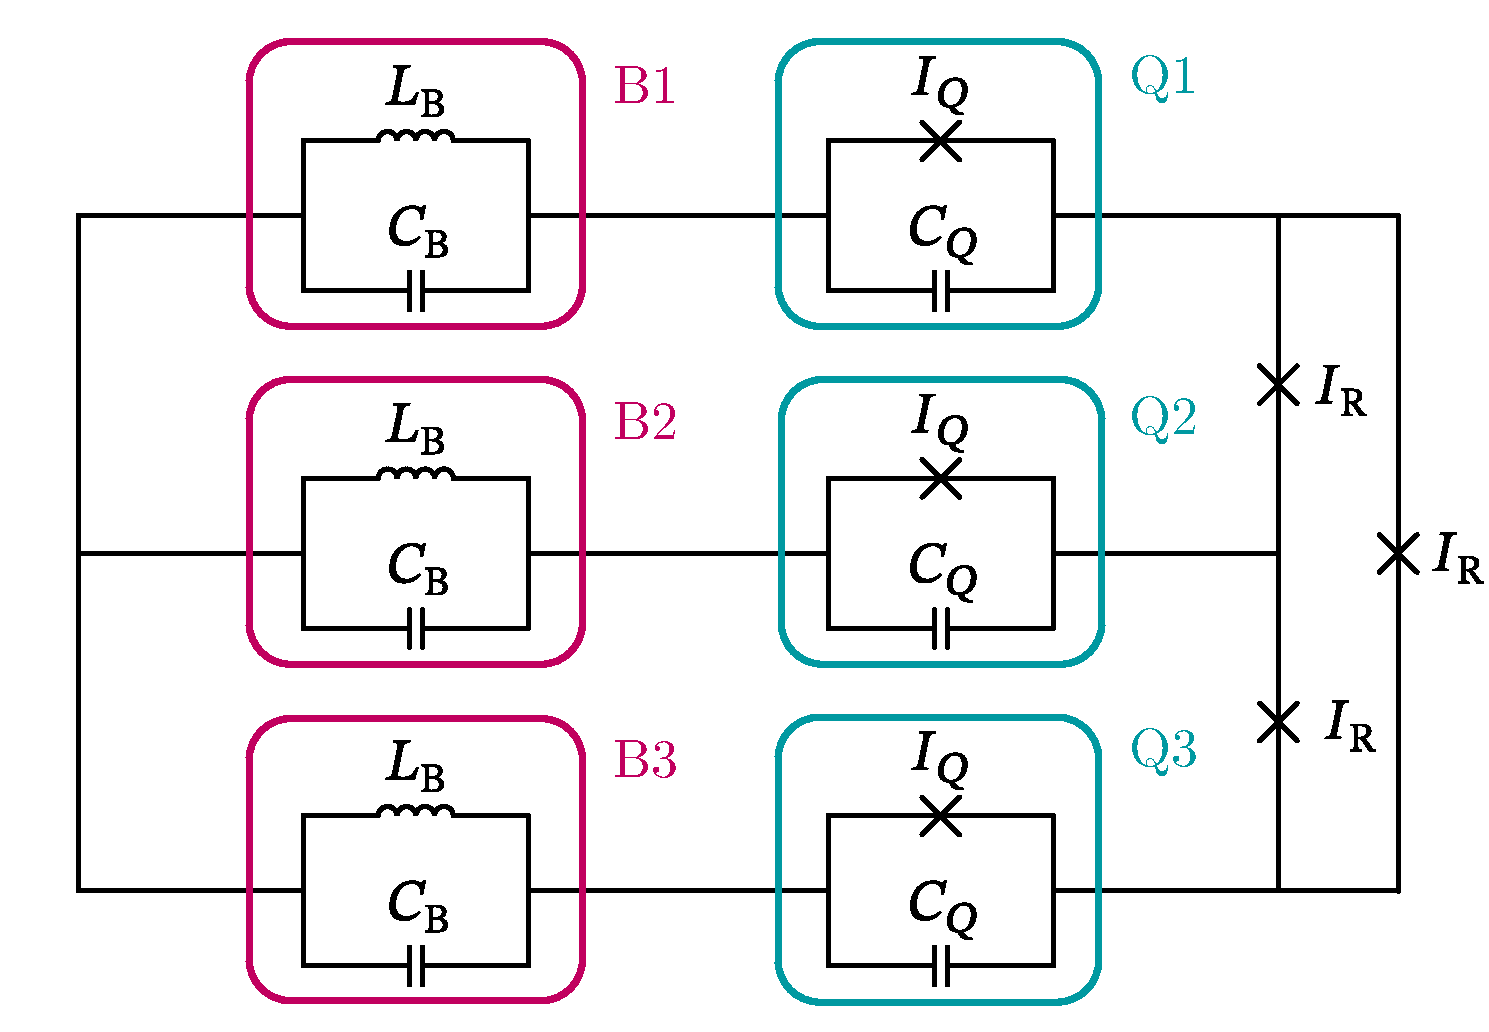
\includegraphics[width=\linewidth]{pics/SC_Rabi_circuit_with_contours.pdf}
  \caption{Superconducting circuit implementation of the two-mode $\Zthree$ Rabi model $H_{\text{R}}$. The LC circuits $(L_{\text{B}}, C_{\text{B}})$ host the boson modes B1, B2, and B3 (marked by the magenta color); the charge qubits $(I_{\text{Q}}, C_{\text{Q}})$ correspond to the qubit degrees of freedom Q1, Q2, and Q3 (marked by the cyan color); Josephson junctions $I_{\text{Rabi}}$ are responsible for the interaction term in the qubit-boson ring. Altogether, the circuit is described by the Hamiltonian~\eqref{eq:physical-hamiltonian}.}
  \label{fig:superconducting-Rabi}
\end{figure}

Next, we argue why this circuit models the Hamiltonian~\eqref{eq:physical-hamiltonian}. Without the coupling JJs, the LC circuits and qubits do not interact with each other and are described by a free Hamiltonian:
\begin{equation}
    H = \sum_{i = 0}^2  H_{\text{LC}, i}(\hat \phi_i, \hat q_i) + \sum_{i = 0}^2 H_{\text{Q},i}(\hat \varphi_i, \hat n_i),
\end{equation}
where $ \hat\phi_i = \hat \Phi_i/\Phi_0$ and $\hat q_i$ are the normalized magnetic flux and  the capacitor charge of the $i$th LC circuit. Here, $\Phi_0 = h/(2e)$ is the magnetic flux quantum with $h$ being the (non-reduced) Planck constant and $e$ -- the electron charge. On the other hand,  $\hat \varphi_i$ and $ \hat n_i$ are the JJ superconducting phase and capacitor charge of the $i$th qubit. The LC circuit Hamiltonian is obviously $ H_{\text{LC}, i} = q_i^2/(2C_{\text{B}}) + \phi_i^2/(2L_{\text{B}})$. We leave the qubit Hamiltonian $H_{Q,i} $ unspecified (beyond it being a charge qubit) so that this framework can accomodate different qubit designs. However, we do require that in the two-dimensional subspace spanned by $|0_i\rangle, |1_i\rangle$, the qubit’s Hamiltonian reduces to a simple $\epsilon\sigma_z$,
\begin{align}
   H_{Q}\bigg|_{\mathcal{V}} = \begin{pmatrix} \bra{0_i} H_Q\ket{0_i} & \bra{0_i} H_Q \ket{1_i} \\ \bra{1_i} H_Q \ket{0_i} & \bra{1_i} H_Q \ket{1_i} \end{pmatrix} = \epsilon \sigma_z,
\end{align}
where the qubit states $\ket{0_i},\ket{1_i}$ are the charge operator eigenstates $ \hat n_i \ket{0_i} = 0 \ket{0_i}, \, \hat n_{i} \ket{1}_i = (N+1)\ket{1}_i$ with $ Q \in \mathbb{Z}$. $\mathcal{V}_i = \operatorname{Span}\{\ket{0_i},\, \ket{1_i}\}$ is the qubit Hilbert space, i.e, a computational subspace of the full Hilbert space of the system implementing the qubit, $H_{Q,i}$.  Due to this property, the operator $ e^{i\hat \varphi_i} $ acts on the qubit subspace $\mathcal{V}_i$ as a raising operator:
\begin{equation}
  \begin{aligned}
    &e^{i\hat\varphi_i}\bigg|_{\mathcal{V}_i} = \begin{pmatrix} \bra{0_i} e^{i\hat\varphi_i} \ket{0_i} & \bra{0_i} e^{i\hat\varphi_i} \ket{1_i} \\ \bra{1_i} e^{i\hat\varphi_i} \ket{0_i} & \bra{1_i} e^{i\hat\varphi_i} \ket{1_i} \end{pmatrix} = \sigma^+,
  \end{aligned}
\end{equation}
because $[e^{i\hat \varphi}, \hat n] = e^{i\hat \varphi}$. 

Connecting the $i$th and $(i+1)$th circuit branches with a JJ closes a superconducting loop. The flux quantization condition for that loop is
\begin{equation}
  \hat \phi_i + \hat\varphi_i + \hat\phi_R - \hat\varphi_{i+1} - \hat\phi_{i+1} = 2\pi N, \, \text{where}\ N \in \mathbb{Z}.
\end{equation} 
In other words, the superconducting phase $\hat \phi_R$ of the coupling JJ is not an independent degree of freedom; it is fixed by the phases of the adjoining nodes. Therefore, for the corresponding term in the Hamiltonian we obtain:
\begin{equation}
\begin{aligned}
    V_{\text{SC QB},j} &= \frac{\Phi_0 I_{\text{R}}}{2\pi}\cos(\hat \phi_R) \\
    &= \frac{\Phi_0 I_{\text{R}}}\cos(\hat \phi_j + \hat \varphi_j - \hat \phi_{j+1} - \hat \varphi_{j+1}).
\end{aligned}
\end{equation}

Projecting this coupling term onto the two-level subspaces of qubits $j$ and $j+1$ yields:
\begin{equation}
\begin{aligned}
    &V_{\text{SC QB},j} \bigg |_{\mathcal{V}_j\otimes \mathcal{V}_{j+1}} = \\
    &=\frac{\Phi_0 I_{\text{R}}}{4\pi}\left(e^{i(\hat\varphi_j - \hat\varphi_{j+1})} e^{i(\hat\phi_j - \hat\phi_{j+1})} + H.c. \right) \bigg|_{\mathcal{V}_j\otimes \mathcal{V}_{j+1}} \\
    &=\frac{\Phi_0 I_{\text{R}}}{4\pi}\left(e^{i(\hat\varphi_j - \hat\varphi_{j+1})} \sigma_j^- \sigma_{j+1}^+ + \mathrm{H.c.} \right).
\end{aligned}
\end{equation}
Here we used the fact that $e^{\pm i\hat\phi}$ acts as a raising/lowering operator for the charge qubit: $e^{i\hat\phi}|_{\mathcal{V}} = \sigma^+$. Hence the need for charge qubits rather than flux or phase qubits.

The Josephson junction coupling between two pairs of an LC circuits and a charge qubits gives us precisely the interaction term we wanted. As a result, we conclude that the system depicted in Fig.~\ref{fig:superconducting-Rabi} is described by the Hamiltonian~\eqref{eq:physical-hamiltonian}.  The qubit-boson ring couplings can be expressed by the circuit parameters:
\begin{equation}
\begin{aligned}
    &\epsilon = \frac{2e^2n_{\mathrm{off}}}{C_Q},\,
    \Omega_{QB} = \frac{1}{\sqrt{L_{\text{B}}C_{\text{B}}}}, \\
    &m_{QB} = \frac{C_{\text{B}}}{4e^2}, \, g = \frac{\Phi_0 I_{\text{R}}}{4\pi}.
\end{aligned}
\end{equation}
Here, the harmonic oscillator mass $m_{\text{QB}}$ has the inverse energy dimension since the charge is normalized. For details of the $\epsilon$ computation, see App.~\ref{app:charge-qubit}. 

Finally, applying the Sec.~\ref{sec:physical-implementation} argument we deduce that the circuit is described by the $\Zthree$ Rabi model. Two practical notes follow from this construction. (i) Replacing each coupling JJ by a dc SQUID makes $g \propto I_{\mathrm{R}}$ tunable (including sign control via flux bias) and allows us to imprint controlled phase offsets around the ring, thereby realizing the ``magnetic'' term with a phase different from Eq.~\eqref{eq:superconducting-magnetic-term}. (ii) The device can be initialized at $g\simeq 0$ with the three qubits and three LC modes effectively decoupled; adiabatic ramp of $g$ then reach the target operating point, while standard dispersive readout on auxiliary resonators provides state discrimination. Taken together, these considerations make the circuit of Fig.~\ref{fig:superconducting-Rabi} a realistic platform for probing $\Zthree$ Rabi model dynamics across coupling regimes without invoking a rotating-wave approximation.


\subsection{Optomechanical implementation}
\label{sec:optomechanical-implementation}

\begin{figure}
    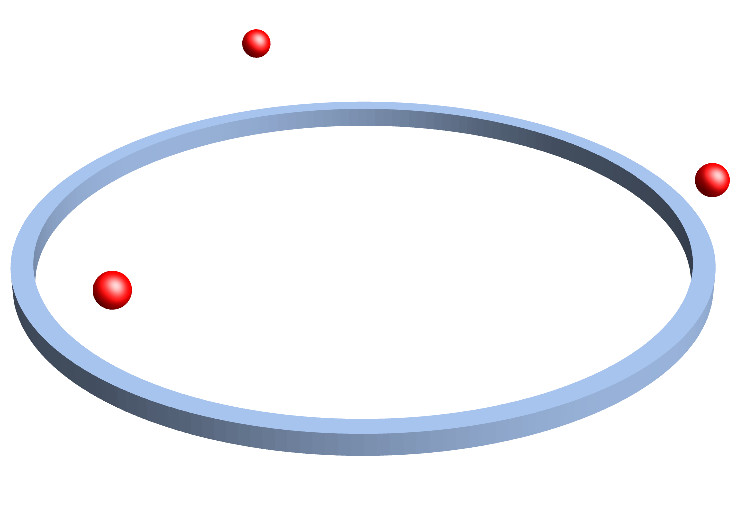
\includegraphics[width=0.8\linewidth]{pics/optomechanical_Rabi_pic.pdf}
    \caption{Schematic illustration of the optomechanical implementation of the two-mode $\Zthree$ Rabi model $ H_{\text{R}'}$ \cite{sedov_chiral_2020} The red spheres are trapped ions carrying two-level systems; their vibrational modes are the bosons from the qubit-boson ring. The blue ring is the chiral waveguide that facilitates the interaction in the qubit-boson ring. The system is described by the Hamiltonian $ H_{\text{OM}}$~\eqref{eq:optomechanical-qb-ring}.}
    \label{fig:optomechanical-rabi}
\end{figure}

Another possible physical platform for the $\Zthree$ Rabi model is an optomechanical system consisting of three spins whose vibrational modes are boson degrees of freedom. They are connected by a chiral circular waveguide that acts as an interaction medium between the spins and the vibrational phonons (first proposed in \cite{sedov_chiral_2020}). Although challenging to realize, this platform illustrates the generality of our approach. In this section, we outline how the $\Zthree$ Rabi model arises in this model, for the extended discussion we refer the reader to the original paper \cite{sedov_chiral_2020}. 

The optomechanical model in question is described by the following Hamiltonian:
\begin{equation}
\label{eq:optomechanical-qb-ring}
\begin{aligned}
    H_{\text{OM}}&=\sum\limits_{k=0}^{\infty} \zeta_k \hat{c}_k^{\dagger} \hat{c}_k + 
 \epsilon \sum_{j=0}^2 \sigma_j^z + \hbar \Omega_{\text{OM}} \sum_{j=0}^2 \hat{b}_j^{\dagger} \hat{b}_j \\
    &+\gamma \sum_{k, j} \left[\sigma_j^{+} \hat{c}_k e^{i k\left[R \phi_j+\hat x_j\right]}+\mathrm {H.c.}\right] \text {, }
\end{aligned}   
\end{equation}
where $\hat c_j^\dagger$ ($\hat c_j$) is the chiral waveguide photon creation (annihilation) operator; $\sigma^z_j$,$\sigma_j^+$, and $\sigma_j^-$ is the ion spin degree of freedom; $\hat b^{\dagger}_j$ ($\hat b_j$) are the ion vibrational phonon creation (annihilation) operators with $\hat x_j = (\hat b_j + \hat b_j^{\dagger})/\sqrt{2}$ being the canonical coordinate operator. The parameters are the following: 
$\zeta_k = v k$ is the waveguide photon dispersion, $\epsilon$ is the spin Zeeman splitting, $\Omega_{\text{OM}}$ is the phonon frequency, and $\gamma$ is the coupling strength.

Using the Schrieffer-Wolff transformation \cite{bravyi_schrieffer_2011}, we can integrate out the photons degrees of freedom to get the Hamiltonian in the form we want:
\begin{equation}
\label{eq:optomechanical-transformed-qb-ring}
\begin{aligned}
&H_{\text{OM,eff}}=  \epsilon \sum_{j=0}^2 \sigma_j^z + \hbar \Omega_{\text{OM}} \sum_{j=0}^2 \hat{b}_j^{\dagger} \hat{b}_j \\
& -\frac{\gamma^2}{2v} \sum_{i<j}\left[i \sigma_i^{+} \sigma_j^- e^{i q R \phi_{i j}} e^{i \eta\left(\hat{b}_i+\hat{b}_i^{\dagger}-\hat{b}_j-\hat{b}_j^{\dagger}\right)}+\mathrm{H.c.}\right].
\end{aligned}
\end{equation}
The Hamiltonian is a bit different from~\eqref{eq:physical-hamiltonian}. It is treated in App. \ref{app:arbitrary-interaction-summary} and gives rise to the following $\Zthree$ Rabi model:
\begin{equation}
\label{eq:optomechanical-rabi}
\begin{aligned}
    &H_{\text{R}'}= - \frac{\gamma^2}{2v} (e^{-5\pi i/6} Z + e^{5\pi i/6} Z^{\dagger}) \\
    &+ \hbar \Omega_{\text{OM}} (\hat a_1^{\dagger} \hat a_1 + \hat a_2^{\dagger} \hat a_2) \\
    &- \frac{\hbar \Omega_{\text{OM}}^{1/2} \eta}{6^{1/2}}\left[(\hat a_1 + \hat a_2^{\dagger}) X  + (\hat a_2 + \hat a_1^{\dagger}) X^{\dagger}  \right]
\end{aligned}
\end{equation}
which differs from the $\Zthree $ Rabi model we acquired in the superconducting circuit context only by the $\Zthree$ ``magnetic'' term's phase $\varphi = - 5\pi/6$.

We can explicitly write down the ``magnetic'' term
\begin{equation}
\label{eq:optomechanical-magnetic-term}
    - \frac{\gamma^2}{2v} (e^{-5\pi i/6} Z + e^{5\pi i/6} Z^2) = \begin{pmatrix}
        \frac{\sqrt{3}\gamma^2}{2v} & 0 & 0 \\ 0 & -\frac{\sqrt{3}\gamma^2}{2v} & 0 \\ 0 & 0 & 0 
    \end{pmatrix}.
\end{equation}
As one can see, the non-zero ``magnetic'' term's phase $\varphi$ leads to all the eigenvalues being non-degenerate. Compare it to Eq.~\eqref{eq:superconducting-magnetic-term}.

As a result the optomechanical system~\eqref{eq:optomechanical-qb-ring} provides another way to realize the $\Zthree$ Rabi model~\eqref{eq:2-mode-z3-Rabi}. This implementation uses the chiral waveguide as a mediator for the qubit-boson interaction $V_{\text{QB}}$~\eqref{eq:physical-hamiltonian}, which is a bit more complicated compared to the superconducting implementation (Fig.~\ref{fig:superconducting-Rabi}). Nevertheless, the optomechanical system~\eqref{eq:optomechanical-qb-ring} still models the Rabi model through the mechanism described in Sec.~\ref{sec:physical-implementation}.



\section{\texorpdfstring{$\Zthree$}{Z3} Potts model}
\label{sec:potts-model}

\subsection{Theoretical description}
\label{sec:theoretical-potts}


The $\Zthree$ Potts model \cite{wu_potts_1982} is a one-dimensional chain of three-level systems, qutrits, with a global $\Zthree$ symmetry. It  originates from statistical physics as a straightforward generalization of the Ising model  \cite{wu_potts_1982,baxter_critical_1982}. Nowadays, the Potts model often appears in the context of qudit quantum computations \cite{aharonov_polynomial_2007,okada_efficient_2019}. However, the direct experimental realization of the Potts model has not yet been achieved. One of the goals of this paper is to propose such an experimental realization using $\Zthree$ Rabi models as building blocks. To achieve this, we generalize the idea of building an Ising model by coupling a chain of $\Ztwo$ Rabi models, proposed by Hwang \cite{hwang_largescale_2013}, to the $\Zthree$-symmetric case.

The $\Zthree$ Potts model Hamiltonian is
\begin{equation}
\begin{aligned}
\label{eq:potts-hamiltonian}
H_{\text{P}} =& f_{\text{P}} \sum\limits_{m=1}^L \left(e^{i\phi}Z_m + e^{-i\phi}Z_m^{\dagger}\right) \\
  &+  J_{\text{P}} \sum\limits_{m=1}^L \left( X_m X_{m+1}^{\dagger} + X_m^{\dagger} X_{m+1}\right),
\end{aligned}
\end{equation}
where $X_m$ and $Z_m$ are the shift and clock matrices~\eqref{eq:shift-clock-matreces} acting on the $m$th qutrit. $f _\text{P}$ describes the strength of a single-site potential, $J_{\text{P}}$ is the coupling strength of $\Zthree$-symmetric nearest-neighbor interaction.

As we have already discussed before, it is difficult to obtain a $\Zthree$ symmetry in an arbitrary three-level system chain. But we have already learned how to construct a $\Zthree$ Rabi model. We use it as a building block for the $\Zthree$ Potts model. We assemble a chain of the $\Zthree$ Rabi models. Then, the three cat-states in the $n$th $\Zthree$ Rabi model~\eqref{eq:three-cat-states} correspond to the three states on the $m$th site of the Potts model $ |j\rangle_m = |\psi_j\rangle_m $ for $j=0,\, 1,\, 2$. In the extreme limit of the Rabi model~\eqref{eq:2-mode-z3-Rabi}, $ \lambda \gg \hbar \Omega_R$,  the higher energy states are effectively decoupled from $|\psi_j\rangle$ states.

The main reason why it is convenient to build the Potts model from the Rabi models is that the boson degrees of freedom in the Rabi model allow us to obtain a $\Zthree$-symmetric interaction. The reasoning is simple: the Rabi model's $\Zthree$ symmetry acting on bosons is a residue of a usual $\mathrm{U(1)}$ boson symmetry. Consequently, if we take a $\mathrm{U(1)}$ symmetric interaction of the boson modes on the neighboring sites in the Rabi model chain, then it is $\Zthree$-symmetric automatically. And the simplest $\mathrm{U(1)}$-symmetric boson interaction is just a hopping term $\hat a_m^{\dagger} \hat a_{m+1} + \textrm{H.c.}$ As a result, to obtain the $\Zthree$ Potts model we need to take a chain of $\Zthree$ Rabi models and couple them by the boson hopping term:
\begin{equation}
\label{eq:coupled-rabi}
\begin{aligned}
    &H_{\text{R chain}} = \\
    &\sum\limits_{m=1}^L H_{\text{R}, m} + J \sum\limits_{m=1}^L \sum\limits_{k=1}^2\left( \hat a_{m,k}^{\dagger} \hat a_{m+1,k} + \hat a_{m+1,k}^{\dagger} \hat a_{m,k}\right),
\end{aligned}
\end{equation}
where $m =1, \dots, L$ indexes the sites of the chain, and $k=1,2$ labels the two boson modes in each $ \Zthree $ Rabi model. We claim that this Hamiltonian gives us precisely the $\Zthree$ Potts model, when we restrict it to the Hilbert space $\bigotimes_n\mathcal{R}_m$ generated by the three cat states on the $m$th site.

Within the Rabi qutrit subspace,  $\hat a_{m,k}$ acts as a permutation between the cat states:
\begin{equation}
    \hat a_{m,k} |\psi_i\rangle_m = (\lambda/\hbar \Omega_{\textrm{R}})|\psi_{i+1}\rangle_m. 
\end{equation}
The action of the creation operator is slightly more complicated:
\begin{equation}
\begin{aligned}
    &\hat a_{m,k}^{\dagger} |\psi_i\rangle_m =  (\lambda/\hbar \Omega_{\textrm{R}})|\psi_{i-1}\rangle_m + \delta,
\end{aligned}
\end{equation}
where $\delta$ is a component orthogonal to the cat-state subspace $\mathcal{R}_n$, which satisfies $\lVert \delta\rVert ^2 = 1$. 
In the extreme coupling~\cite{kozin_cavityenhanced_2025,KozinMiserevSchottky} regime $\lambda/\hbar \Omega_{\text{R}} \gg 1$, we can neglect $\delta$. As a result, within the Rabi qutrit subspace $\mathcal{R}_n$, the creation (annihilation) operator act as cyclic permutation operator, $\hat a_{m,k}^{\dagger}|_{\mathcal{R}} \approx (\lambda/\hbar \Omega_{\textrm{R}}) X^{\dagger}$ ($\hat a_{m,k}|_{\mathcal{R}} = (\lambda/\hbar \Omega_{\textrm{R}}) X$). Consequently, in this sector the coupled Rabi chain is equivalent to the Potts model:

\begin{equation}
\begin{aligned}
    J &\sum\limits_{k=0}^{2} \left(\hat a_{m,k}^{\dagger} \hat a_{m+1,k} + \hat a_{m+1,k}^{\dagger} \hat a_{m,k}\right) = \\
    &3(\lambda/\hbar \Omega_{\textrm{R}})^2 J\left(X_m^{\dagger} X_{m+1} + X_{m+1}^{\dagger} X_m\right).
\end{aligned}
\end{equation}
In summary, a chain of $\Zthree$ Rabi models coupled by boson hopping implements the nearest-neighbor term of the $\Zthree$ Potts Hamiltonian exactly within the qutrit formed by the $\Zthree$ Rabi cat states~\eqref{eq:three-cat-states}. The $\Zthree$-symmetric nearest-neighbor coupling strength is $J_{\text{P}} = 3(\lambda/\hbar \Omega_{\textrm{R}})^2 J$. While the single-site term $f_{\text P}(e^{i\phi}Z_m+\mathrm{H.c.})$ comes from the small energy splitting of the $\Zthree$ cat states [Eq.~\eqref{eq:rabi-spectrum}], which is controlled by the parameter $B$. The mapping requires to be in the extreme coupling regime $\lambda/\hbar \Omega_{\mathrm R}\gg 1$ and the scale separation $J_{\text P},f_{\text P}\ll \hbar \Omega_{\text{R}}$. 

\subsubsection{Qubit-boson-ring point of view}
\label{sec:underlying-qb-ring}

 In the previous section, we showed how to construct the $\Zthree$ Potts model out of a chain of $\Zthree$ Rabi models. However, each Rabi model is itself implemented by a QB ring [see Sec.~\ref{sec:physical-implementation}]. Here, we show how these QB rings should be coupled to get the boson-hopping interaction~\eqref{eq:coupled-rabi} for the Rabi models. It turns out to be rather straightforward. The hopping term between the QB ring bosons $\hat b_{m,j}$ and $\hat b_{m,j}^{\dagger}$ give us precisely the hopping term between the $\Zthree$ Rabi model bosons $\hat a_{m,k}$ and $\hat a_{m,k}^{\dagger}$ since the Fourier transform does not change the form of the boson hopping interaction:
\begin{equation}
\begin{aligned}
    &\sum\limits_{j=0}^2 \left(\hat b_{m,j}^{\dagger} \hat b_{m+1,j} + \hat b_{m+1,j}^{\dagger} \hat b_{m,j}\right) \\
    =&\sum\limits_{k=0}^{2} \left(\hat b_{m}^{\dagger}(k) \hat b_{m+1}(k) + \hat b_{m+1}^{\dagger}(k) \hat b_{m}(k)\right),
\end{aligned}
\end{equation}
where $\hat b_{m}(k)$ and $\hat b_m^{\dagger}(k)$ are the Fourier transformed QB ring boson modes. But we know that the Rabi model boson modes are precisely the first and the second their components, $\hat a_{m,k} = \hat b_m(k)$ and $\hat a_{m,k}^{\dagger} = \hat b_m(k)$ for $k =1,2$ [see Eq.~\eqref{eq:effective-rabi}]. Therefore, we obtain precisely the interaction~\eqref{eq:coupled-rabi} we wanted. Also, we have a hopping term for the extra boson mode $\hat b_{m}(0), \hat b^{\dagger}_{m}(0)$, which decouples the same way it did in Sec. \ref{sec:physical-implementation}.

The couplings in the Potts Hamiltonian can be related to the underlying QB ring parameters. In fact: 
\begin{equation}
\begin{aligned}
    &f_{\text{P}} = g \exp\left(-\frac{1}{2 \hbar m_{QB} \Omega_{\text{QB}}}\right),\\
    &J_{\text{P}} = \frac{J }{2\hbar m_{\text{QB}} \Omega_{\text{QB}}}.
\end{aligned}
\end{equation}

As a result, the $\Zthree$ Potts model can be indeed implemented by a chain of the QB ring units, each implementing the $\mathbb{Z}_3$ Rabi model. This system is realistic in an experimental setup. Below, we illustrate our idea with the corresponding superconducting circuit (Fig.\ref{fig:superconducting-potts}).

\subsection{Coupled superconducting \texorpdfstring{$\Zthree$}{Z3} Rabi models as the Potts model}


\begin{figure}[t]
    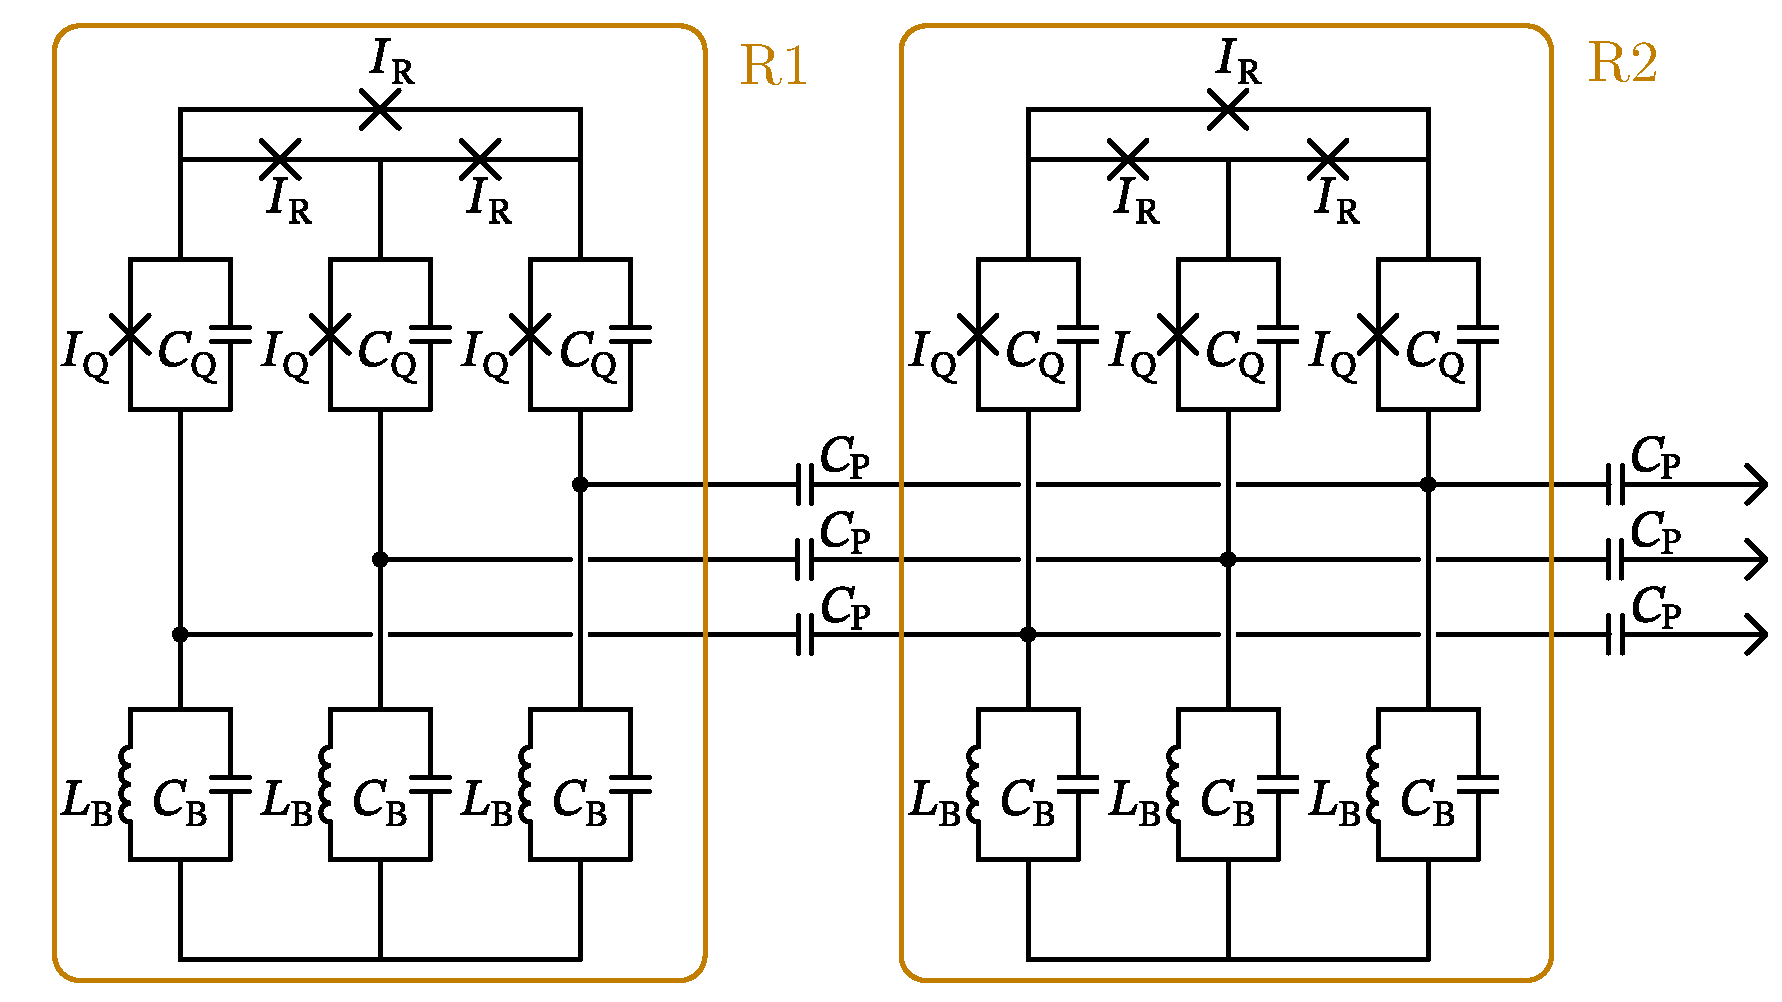
\includegraphics[width=\linewidth]{pics/SC_Potts_circuit_with_contours.pdf}
    \caption{Superconducting circuit implementation of the Potts model. It is composed from a chain of the $\Zthree$ Rabi model superconducting circuits $\mathrm{R1}$, $\mathrm{R2}$, etc [see Fig.~\ref{fig:superconducting-Rabi}]. The Potts model circuit is described by the Hamiltonian~\eqref{eq:coupled-rabi}. Subscript ``B'' denote elements corresponding to boson degrees of freedom; subscript ``Q'' denote qubit elements; subscript ``R'' denote elements responsible for interaction in qubit-boson ring; subscript ``P'' denote elements responsible for interaction in Potts model.}
    \label{fig:superconducting-potts}
\end{figure}

Having explored the theoretical construction of the Potts model based on a chain of the Rabi models, here we show how to implement the Potts model using superconducting circuits. We consider a chain of the superconducting circuits simulating the $\Zthree$ Rabi models [see Sec.~\ref{sec:superconducting-implementation}]. Next, we need to couple the neighboring Rabi models with a boson hopping term to get the Hamiltonian~\eqref{eq:coupled-rabi}. As we have learned in Sec.~\ref{sec:underlying-qb-ring}, we must couple the bosons modes of the neighboring QB rings pairwise to achieve this. Therefore, we connect the corresponding LC circuits of the neighboring QB rings by the capacitive coupling (Fig.~\ref{fig:superconducting-potts}). Although nearest-neighbor capacitive coupling induces an all-to-all coupling after introducing the canonically-conjugated momentum \cite{forschungszentrumjulichgermany_lecture_2024}, we can ignore that assuming that the capacitance responsible for the coupling of the nearest-neighbor Rabi models is much smaller than the cavity capacitance, $C_{\text{P}} \ll C_{\text{B}}$. In this limit, the nearest-neighbor coupling turns out to be proportional to $C_{\text{P}}/C_{\text{B}}^2$, capacitors are:
\begin{align}
    &V_{\text{P},m,j} = \\
    &-\frac{C_{\text{P}}}{2C_{\text{B}}^2} (\hat q_{m+1,j} - \hat q_{n,j})^2 = -\frac{2e^2C_{\text{P}}}{C_{\text{B}}^2}\left(\hat n_{m,j}^2 + \hat n_{m+1,j}^2\right)\nonumber\\
    &- \frac{e^2\hbar m_{\text{QB}}\Omega_{\text{QB}}C_{\text{P}}}{C_{\text{B}}^2}\left(\hat b^{\dagger}_{m,j} \hat b^{\dagger}_{m+1,j} - \hat b^{\dagger}_{m,j} \hat b_{m+1,j} + \mathrm{H.c.}\right)\nonumber
\end{align}

where we expressed the charge $\hat q_{m,j}$ through the creation and annihilation operators, $\hat q_{m,j} = 4e^2\hat n_{m,j} = i4e^2(\hat b_{m,j}^{\dagger} - \hat b_{m,j})\sqrt{\hbar m_{\text{QB}} \Omega_{QB}/2}$.
\begin{comment}
\begin{align}
    &V_{\text{P},n,j} = \frac{1}{2L_{\text{P}}} (\hat \Phi_{n+1,j} - \hat \Phi_{n,j})^2 = \Phi_0^2\frac{\hat \phi_{n,j}^2 + \hat \phi_{n+1,j}^2}{2L_{\text{P}}} \\
    &- \Phi_0^2\frac{\hat b^{\dagger}_{n,j} \hat b^{\dagger}_{n+1,j} + \hat b^{\dagger}_{n,j} \hat b_{n+1,j} + \hat b_{n,j} \hat b^{\dagger}_{n+1,j} + \hat b_{n,j} \hat b_{n+1,j}}{4\hbar L_{\text{P}}m_{\text{QB}}\Omega_{QB}} \notag
\end{align}
where we expressed the flux operator through the creation and annihilation operators, $\hat \Phi_{n,j} = \Phi_0\hat \phi_{n,j} = (\hat b_{n,j} + \hat b_{n,j}^{\dagger})\Phi_0/\sqrt{2\hbar m_{\text{QB}} \Omega_{QB}}$.
\end{comment}

We ignore the $ \hat n_{m,j}^2 $ and $ \hat n_{m+1}^2 $ terms because they simply renormalize the Rabi model parameters. Additionally, the capacitor coupling produces undesired terms $\hat b^{\dagger}_{n,j} \hat b^{\dagger}_{n+1,j}$ and $\hat b_{n,j} \hat b_{n+1,j}$. However, we can use the Rotating Wave Approximation (RWA) to eliminate them. For RWA to be applicable, we require $\hbar\Omega_{QB} \gg e^2\hbar m_{\text{QB}}\Omega_{\text{QB}}C_{\text{P}}/C_{\text{B}}^2$, or after the simplification it turns out to be equivalent to $C_{\text{P}} \ll C_{\text{B}}$ After applying RWA, we are left precisely with the hopping term between the boson modes of the neighboring Rabi models. Consequently, in line with Sec.~\ref{sec:theoretical-potts} the superconducting circuit in Fig.~\ref{fig:superconducting-potts} models the $\Zthree$ Potts model. The coupling parameters of the resulting Potts model could be expressed through the circuit parameters:
\begin{equation}
\begin{aligned}
    &f_{\text{P}} = \frac{\Phi_0I_{\text{R}}}{4\pi} \exp\left(-\frac{2e^2}{\hbar}\sqrt{\frac{L_{\text{B}}}{C_{\text{B}}}}\right), \\
    &J_{\text{P}} = \frac{e^2 C_{\text{P}}}{2C_{\text{B}}^2}. 
\end{aligned}
\end{equation}

In this section, we proposed the superconducting circuit (Fig.~\ref{fig:superconducting-potts}) that simulates the $\Zthree$ Potts model. The necessary parameter range includes: 
\begin{enumerate}[label=(\roman*)]
    \item Rabi extreme coupling regime, 
    \begin{equation}
    \tag{\theequation .A}
    \sqrt{\frac{2\hbar e^2}{3L^{1/2}_{\text{B}}C^{3/2}_{\text{B}}}} \ll 1;
    \end{equation}
    \item Potts model parameters keeping the dynamics within the cat-state qutrit, 
    \begin{equation}
    \tag{\theequation .B}
    \begin{aligned}J_{\text{P}}=\frac{e^2 C_{\text{P}}}{2C_{\text{B}}^2}&\ll \frac{\hbar}{\sqrt{L_{\text{B}}C_{\text{B}}}}, \\
    f_{\text{P}} = \frac{\Phi_0I_{\text{R}}}{4\pi} \exp\left(-\frac{2e^2}{\hbar}\sqrt{\frac{L_{\text{B}}}{C_{\text{B}}}}\right) &\ll \frac{\hbar}{\sqrt{L_{\text{B}}C_{\text{B}}}};
    \end{aligned}
    \end{equation}
    \item RWA being valid, and the capacitive coupling being local, 
    \begin{equation}
    \tag{\theequation .C}
    \frac{C_{\text{P}}}{C_{\text{B}}} \ll 1.
    \end{equation}
\end{enumerate} 
All these requirement should be feasible for an actual superconducting circuit. As a result, we believe that our setup should be possible to implement experimentally.


\subsection{Coupled optomechanical \texorpdfstring{$\Zthree$}{Z3} Rabi models as the Potts model}

\begin{figure}[t]
    \centering
    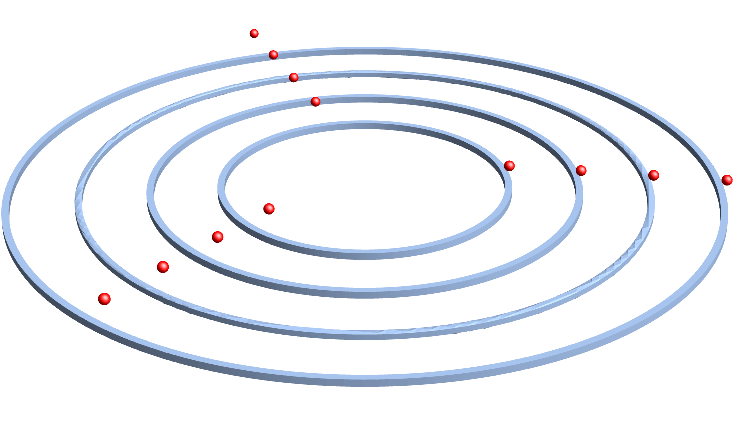
\includegraphics[width = 0.8 \linewidth]{pics/optomechanical_Potts_pic.pdf}
    \caption{Schematic illustration of the optomechanical (OM) implementation of the Potts model. It consists of several concentric OM implementations of the Rabi model, i.e., several concentric cyclic chiral waveguide and three trapped ions on top of each waveguide.}
    \label{fig:optomechanical-potts}
\end{figure}

We can, in principle, construct an optomechanical implementation of the $\Zthree$ Potts model by similarly coupling multiple $\Zthree$ Rabi units. However, the geometry is a bit more peculiar due to the use of a circular waveguide in the optomechanical Rabi setup. To build the optomechanical $\Zthree$ Potts model we arrange the optomechanical $\Zthree$ Rabi model concentrically (see Fig. \ref{fig:optomechanical-potts}). On the one hand, the radius of the waveguide does not affect the parameters of the model, on the other hand, placing the ions of the neighboring Rabi models close to each other generates an effective phonon-phonon interaction via the Coulomb interaction \cite{schneider_experimental_2012,timm_dynamics_2023}. The phonon-phonon coupling between the neighboring Rabi models leads to the same effective Hamiltonian~\eqref{eq:coupled-rabi}, realizing the $\Zthree$ Potts model as described before.


\subsection{Chiral Potts model and parafermions}

In this subsection, we briefly review the chiral $\Zthree$ Potts model. It is a generalization of the ordinary $\Zthree$ Potts model that has a chiral nearest-neighbor interaction:
\begin{equation}
\label{eq:chiral-potts-hamiltonian}
\begin{aligned}
    H_{\text{chP}} = &f'\sum_{n=1}^L (e^{i\phi'} Z_n + e^{-i\phi'} Z_n^{\dagger}) \\
    &+ J' \sum (e^{i\theta'} X_n X_{n+1}^{\dagger} + e^{-i\theta'} X_n^{\dagger} X_{n+1}).
\end{aligned}
\end{equation}
In other words, it is simply the $\Zthree$ Potts model~\eqref{eq:potts-hamiltonian} with a complex nearest-neighbor coupling $J'e^{i\theta'}$. 

In the construction described in Sec.~\ref{sec:potts-model}, the interaction parameter $J'$ originates from the boson interaction of the neighboring QB rings. Hence, if we want to engineer the chiral Potts model, we have to find a way to create the chiral boson-hopping term. A chiral boson coupling arises when hopping between boson modes acquires a complex amplitude, so that excitations accumulate a nontrivial phase when moving around a closed loop. In general, such a complex hopping term
\begin{equation}
H_{nm} = g \, e^{i\phi_{nm}} \hat a_n^\dagger \hat a_m + \mathrm{H.c.}
\end{equation}
corresponds to a synthetic gauge field, with the directed phase factors $\phi_{nm}$ acting as Peierls phases. The net phase around a plaquette defines an effective magnetic flux that breaks time-reversal symmetry and leads to chiral transport of photons or phonons.

In trapped-ion arrays, the bosons are vibrational phonons. Coupling between the phonons is engineered through Coulomb interaction combined with laser-induced forces. By introducing a static gradient in trap frequencies and applying periodic modulation (photon-assisted tunneling), the effective phonon hopping becomes resonant and inherits the phase of the driving field. Adjusting laser phases thus imprints controlled Peierls phases on the phonon couplings, producing synthetic fluxes that enable chiral phonon propagation \cite{bermudez_synthetic_2011, schneider_experimental_2012a,vermersch_implementation_2016,roushan_chiral_2017,kiefer_floquetengineered_2019,bazavan_synthetic_2024}.

In superconducting circuits, the bosons are microwave photons in resonators or qubits. Here, Josephson junctions provide nonlinear couplers whose effective interaction strength can be modulated parametrically by flux or multi-tone microwave pumping. When the pump frequency matches the detuning between two modes, frequency-converting tunneling occurs with an amplitude set by the pump strength and a phase set by the pump phase. Embedding such complex hoppings in a ring of modes yields a net synthetic magnetic flux, leading to unidirectional photon circulation \cite{kapit_quantum_2013,sliwa_reconfigurable_2015,gu_microwave_2017, cao_parametrically_2024}.


Assuming that we obtained the chiral coupling in one of the ways described above, now we want to discuss what physical effects the complex coupling causes in the Potts model. The most interesting consequence is the parafermion physics. The duality between the Potts model and the parafermion chain is the generalization of the duality between the Ising model and Kitaev chain that displays Majoranas \cite{kitaev_unpaired_2001}. Similarly to the Ising model, there is a generalization of the Jordan-Wigner transformation. It is called the Fradkin-Kadanoff (FK) transformation \cite{fradkin_disorder_1980}, and it maps the qutrit operators $X_j$ and $ Z_j$ to the parafermions operators:
\begin{equation}
\Gamma_j = \prod\limits_{k<j} Z_k X_j , \quad \Delta_j = \prod\limits_{k\le j} Z_k X_j.
\end{equation}
Here $\Gamma_j, \, \Delta_j$ are parafermion operators with a parafermion commutation relation: $\Gamma_j \Gamma_k = \omega^{\sgn(j-k)} \Gamma_k \Gamma_j, \, \Delta_j \Delta_k = \omega^{\sgn(j-k)} \Delta_k \Delta_j$, and finally $\Gamma_j \Delta_k = \omega^{\sgn(j-k)} \Delta_k \Gamma_j$.

Using the FK transformation, it is easy to show that the Potts model is equivalent to a parafermion chain. The only problem is that FK transformation is not local. In terms of parafermion operators, the chiral Potts model Hamiltonian~\eqref{eq:chiral-potts-hamiltonian} looks like 
\begin{equation}
\begin{aligned}
    H_{\text{chP}} = &f' \sum \left( e^{i\phi'} \Gamma_j \Delta_j^{\dagger} + e^{-i\phi'} \Delta_j \Gamma_j^{\dagger}\right) \\
    &+J' \sum \left(e^{i\theta'} \Delta_j \Gamma_{j+1}^{\dagger} + e^{-i\theta'} \Gamma_{j+1} \Delta_j^{\dagger}\right).
\end{aligned}
\end{equation}

On the other hand, it is well-known that parafermion chain hosts a topological phase with the parafermion edge modes  \cite{fendley_parafermionic_2012}:
\begin{equation}
\label{eq:parafermion-edge-mode}
\Gamma_{\text{edge}} = \Gamma_1 + \frac{f'}{J' \sin(3\theta')} \mathcal{O} + \dots,
\end{equation}
where the dots represent higher order terms.
This expression also clarifies why we required the chiral coupling~\eqref{eq:chiral-potts-hamiltonian}. For the parafermion edge mode to be localized, the expansion parameter must satisfy $f'/(J'\sin(3\theta')) < 1$. In the non-chiral case, however, $\theta' = 0 $, so the expansion parameter diverges, $f'/(J'\sin(3\theta')) = \infty$.

While the chiral Potts model allows us to simulate the parafermion physics, after the FK transformation the parafermion edge mode is not localized. As a result, we do not have an actual topological phase in the chiral Potts model. However, having the exact mapping between the parafermion chain and the Potts model is still valuable, as it provides an insight into parafermion behavior even in the absence of a true topological phase.



\section{Conclusion}
\label{sec:conclusion}
We established a hierarchy of $\Zthree$-symmetric models. First, we link a qubit–boson ring to an effective $\Zthree$ Rabi model. Then, we assemble a chain of $\Zthree$ Rabi models, each hosting an individual qutrit degree of freedom. The resulting chain simulates the $\Zthree$ Potts model. In the ring, the $\Zthree$ symmetry appears as a discrete rotation; upon projecting to the single-excitation manifold, it acts as an internal symmetry that is inherited by the coupled-block construction of the $\Zthree$ Potts Hamiltonian.

Our main goal was to suggest a way towards an experimental realization of the $\Zthree$ Rabi and Potts models. The superconducting circuit we proposed is experimentally feasible. However, this approach does not have to be limited only to the superconducting circuit platform. For example, we believe that a similar strategy could work for the spin-qubit systems, though this remains a topic for future research.

More broadly, our work highlights the intriguing potential of $\Zn$-symmetric systems within condensed matter physics. These systems present a fertile ground for discovering novel quantum phenomena, many of which remain to be fully understood or described.



\section*{Acknowledgments} 

We thank Daria Kalacheva, Henry Legg, Katharina Laubscher, and Ilia Luchnikov for fruitful discussions and useful comments. This work was supported as a part of NCCR SPIN, a National Centre of Competence in Research, funded by the Swiss National Science Foundation (grant number 225153). This work has received funding from the Swiss State Secretariat for Education, Research and Innovation (SERI) under contract number M822.00078.


\appendix

\section{QB ring generalization to an arbitrary interaction matrix}
\label{app:arbitrary-interaction-summary}

In this appendix, we summarize how the Sec.\ref{sec:physical-implementation} derivation extends to a QB ring
with an arbitrary relative interaction strength between different qutrit-boson pairs that is still $\Zthree$-symmetric. We consider a Hamiltonian that is a generalization of the Hamiltonian given in Eq.~\eqref{eq:physical-hamiltonian},
\begin{equation}
\label{eq:arbitary-interaction-hamiltonian}
  \begin{aligned}
    H_{\text{gen}} &= \epsilon \sum_{j=1}^{3} \sigma_j^z
      + \hbar \Omega \sum_{j=1}^{3} \hat a_j^{\dagger} \hat a_j + V_{\text{gen}},
      \\
    V_{\text{gen}} &= g \sum_{j,k=1}^3 A_{jk}
      \sigma_j^{+} \sigma_k^{-} e^{ i ( \hat x_j - \hat x_k ) },
  \end{aligned}
\end{equation}
with the interaction matrix being Hermitian, $A^{\dagger}=A$. Applying the same sequence of steps as in Sec.~\ref{sec:physical-implementation}, i.e., the momentum translation $S$,
the Fourier transform, the restriction to $\mathcal H_{\text{QB},1}$, and the final basis transforms, leads to the Hamiltonian~\eqref{eq:effective-rabi}. However, the purely spin term is now equal to $gHAH^{\dagger}$ instead of $g(Z+Z^{\dagger})$ previously, where $H$ is the Hadamard matrix. Taking into account that $A$ commutes with the $\Zthree$ symmetry and is Hermitian, it can be mapped onto the
canonical $\Zthree$ Rabi model term, $g HAH^{\dagger}= \tilde g(e^{i\phi} Z + e^{-i\phi}Z^{\dagger})$, where $\tilde g$ and $\phi$ depend on the matrix $A$.  

In the superconducting implementation, one has $A = X + X^{\dagger}$, thereby
recovering the special case treated in Sec.~\ref{sec:physical-implementation}. On the other hand, the optomechanical realization of the QB ring~\eqref{eq:optomechanical-transformed-qb-ring}
gives rise to a different interaction matrix $A = -iX + iX^{\dagger}$. However, the logic is exactly the same. As a result, in the optomechanical implementation of the $\Zthree$ Rabi model we obtain a different phase for the qutrit term, $g HAH^{\dagger} = g(e^{-5\pi i/6} Z + e^{5\pi i/6} Z^{\dagger})$ [see Eqs.~(\ref{eq:optomechanical-rabi},\ref{eq:optomechanical-magnetic-term})].





\section{Charge qubit for the \texorpdfstring{$\Zthree$}{Z3} Rabi model}
\label{app:charge-qubit}


\begin{figure}[t]
    \centering
    \subfloat[]{
         \centering
         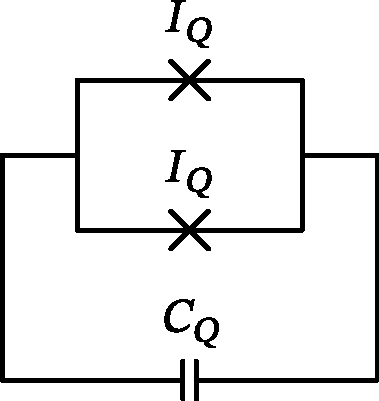
\includegraphics[width=0.4\linewidth]{pics/SC_qubit2_svg-tex.pdf}
         \vspace{0.1pt} %% Shifts the first image to allign it with x axis of the second image
         %%\caption{}
         \label{fig:2nd-harmonic-qubit-a}}
     \hfill
    \subfloat[]{
         \centering
         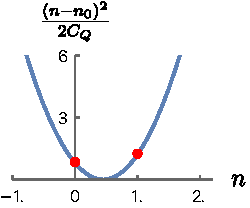
\includegraphics[width=0.5\linewidth]{pics/capacitor_potential.pdf}
         %%\caption{ }
         \label{fig:second-harmonic-qubit-b}}
    \caption{Second-harmonic qubit. a) The electric circuit of the second-harmonic qubit circuit. b) The capacitor potential~\eqref{eq:second-harmonic-qubit} for $n_0 = 0.45 = 0.5 - 0.05 $. The red dots show the eigenenergies of the second-harmonic qubit.}
    \label{fig:second-harmonic-qubit}
\end{figure}

Here we provide details on the superconducting qubit used in Sec.~\ref{sec:superconducting-implementation}. While the Cooper Pair Box (CPB) qubit is probably the most well-known type of charge qubit, it is not suitable for our purposes because its eigenstates are not charge states but rather their symmetric/antisymmetric superpositions. In other words, the CPB Hamiltonian is proportional to $\sigma^x$ in the charge basis. This is undesirable because it causes the qubit chain Hamiltonian to fail to commute with the total qubit-excitation-number operator $S^z$.



\begin{figure*}[th]
    \captionsetup[subfloat]{captionskip=-135pt} %%Moving captions on top
    \centering
    \subfloat[]{
         \centering
         %%\caption{}
        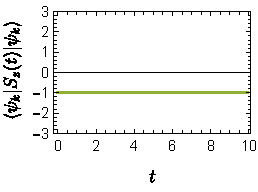
\includegraphics[width=0.32\linewidth]{pics/Spin_correlators_1.pdf}
         \label{fig:1st-spin-correlator}}
    \subfloat[]{
         \centering
        %%\caption{ }
        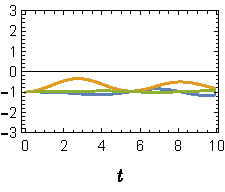
\includegraphics[width=0.274\linewidth]{pics/Spin_correlators_2.pdf}
         \label{fig:2nd-spin-correlator}}
    \subfloat[]{
         \centering
        %%\caption{}
        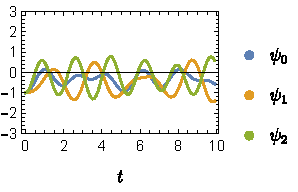
\includegraphics[width=0.37\linewidth]{pics/Spin_correlators_3.pdf}
         \label{fig:3rd-spin-correlator}}
    \caption{Time dependence of the $z$-component of the total spin operator. To illustrate robustness of the Rabi model implementation with the respect to the disorder~\eqref{eq:rabi-breaking-disorder} we plotted $\langle S^z(t) \rangle$. The standard variance of the disorder $\Delta_j$  equals for plot a) $ 0.1\, \Omega_{\text{QB}}$; b) $0.3\,\Omega_{\text{QB}}$; c) $1\,\Omega_{\text{QB}}$.}
    \label{fig:spin-excitation-plot}
\end{figure*}



Hence, we need another type of charge qubit. Considering that the $\sigma^x$ term in the Hamiltonian arises from the JJ term, removing which, we would have a Hamiltonian proportional to $\sigma^z$ in the charge basis. While it solves the symmetry issue, such a system cannot be called a qubit because of the absence of the non-linearity.

Consequently, we want two things simultaneously: (i) the Hamiltonian proportional to $\sigma^z$ in the charge basis, and (ii) JJ that provides the non-linearity being present in the qubit circuit. The solution turns out to be a higher harmonic Josephson junction. Usually it is neglected, but the JJ Hamiltonian always includes higher harmonics as well,
\begin{equation}
    H_{JJ} = E_{J,1} \cos{\hat \phi} + E_{J,2} \cos{2\hat \phi} + \dots,
\end{equation}
where $\phi$ is the superconducting phase.

In practice, the higher harmonics are usually considerably weaker, $E_{J,2} \ll E_{J,1}$. However, if we eliminate the first harmonic completely, only the second harmonic is left. The second harmonic, on the one hand, can help to suppress the noise and, on the other hand, does not induce any coupling in the qubit subspace:
\begin{equation}
    \cos{2\hat \phi}\bigg|_{\mathcal{V}} = \frac{1}{2}\left(e^{2i\hat\phi} + e^{-2i\hat \phi}\right)\bigg|_{\mathcal{V}}=\frac{1}{2}\left((\sigma^+)^2 + (\sigma^-)^2\right) =0
\end{equation}

To eliminate the first harmonic, we can use a Superconducting Quantum Interference Device (SQUID) \cite{valentini_parityconserving_2024}. If the magnetic flux through the SQUID is tuned to $\Phi = \pi$, then the SQUID Hamiltonian looks like,
\begin{equation}
\begin{aligned}
    H_{\text{SQUID}} = &I_{Q,1} \cos(\hat \phi) + I_{Q,2} \cos(2\hat \phi) + I_{Q,1} \cos(\hat \phi + \pi) \\
    &+ I_{Q,2} \cos(2\hat \phi + 2\pi) = 2 I_{Q,2} \cos(2\hat \phi).
\end{aligned}
\end{equation}
As a result, only the second harmonic is left.

Consequently, we can construct a qubit based on the second-harmonic JJ (see Fig. \ref{fig:second-harmonic-qubit}). It is described by the Hamiltonian:
\begin{equation}
\label{eq:second-harmonic-qubit}
    H = \frac{1}{2C_{\text{Q}}} (\hat n - n_0)^2 + 2 I_{\text{Q},2} \cos(2\hat\phi)
\end{equation}
By biasing the offset charge slightly away from the symmetric point ($n_0 = 0.5 - n_{\mathrm{off}}$ with $n_{\mathrm{off}} \ll 1$), the low-energy Hamiltonian of the qubit is
\begin{equation}
    H_{\text{Q}} = \frac{n_{\mathrm{off}}}{2 C_{\text{Q}}} \sigma^z.
\end{equation}
Hence, we obtain the qubit Hamiltonian proportional to $\sigma_z$ as desired. Here we assume that $\frac{1}{2C_{\text{Q}}} \gg 2 I_{\text{Q},2}$, i.e., the charging energy dominates over the Josephson energy, as is usually the case for charge qubits.

To conclude, the charge qubit we have in mind consists of a capacitor and the second-harmonic JJ. One can think of it as a modified version of a Cooper Pair Box qubit. Here, we only briefly described its blueprint to further support the implementation proposed in Sec.~\ref{sec:superconducting-implementation}.


\section{Disorder in the superconducting implementation of the \texorpdfstring{$\Zthree$}{Z3} Rabi model}
\label{app:disorder}
\subsection{Disorder breaking \texorpdfstring{$S^z$}{Z\^z} conservation}

First, while discussing the effects of disorder on the qubit-boson ring~\eqref{eq:physical-hamiltonian}, we must consider a term that breaks the conservation of the total excitation number of qubits $\hat S^z$. This conservation law is broken by small misalignments of the Zeeman terms with the $\hat z$ direction:
\begin{equation}
    H_{\text{QB,dis}} = H_{\text{QB}} + \sum_{j=1}^3 \Delta_j \sigma^x_{j}.
\end{equation}
As explained in App. \ref{app:charge-qubit}, $\Delta_j$ being equal to zero for qubit-boson ring based on superconducting circuits relies on the fine-tuning of the SQUID magnetic field. Therefore, in a realistic setting some small detuning is inevitable, $\Delta_j = I_{Q,1}\sin(\Delta \Phi_j)$.

As a result, the Hamiltonian no longer commutes with $S^z$ operator, $[H_{QB,\text{dis}}, S^z] \neq 0 $. This means that the exact mapping to the $\Zthree$ Rabi model derived earlier does not hold anymore. However, assuming that the disorder is considerably smaller than other parameters in the Hamiltonian, we can still hope that the dynamics remains approximately that of the Rabi model. An analytic estimate is cumbersome, so we performed numerical simulations of the qubit–boson ring. The results are shown in Fig. \ref{fig:spin-excitation-plot}. The figure shows the time evolution of $\langle S^z(t)\rangle$ for various disorder strengths. The simulation indicates that for small disorder the qubit-boson ring's evolution stays near the single excitation subspace $\mathcal{H}_1$ as $\langle S^z \rangle(t) \approx -1$ throughout. We speculate that even when $S^z$ is not strictly conserved, the system’s spins collectively precess around the $S^z=-1$ direction, effectively keeping $\langle S^z \rangle$ near $-1$. 



\subsection{Disorder breaking \texorpdfstring{$\Zthree$}{Z3} symmetry}

Now, assuming that $S^z$ conservation is maintained ($\Delta_j=0$), we now examine a different type of disorder: spatial variations in the system parameters . In an inhomogeneous qubit–boson ring, the $\Zthree$ symmetry is obviously broken. However, we want to identify explicitly which term in the effective Rabi Hamiltonian this symmetry breaking corresponds to.
\begin{equation}
\label{eq:rabi-breaking-disorder}
\begin{aligned}
  H_{\text{QB}}' &= \sum_j \epsilon_{j} \sigma_j^z + \sum_j \hbar \Omega_{\text{QB},j} \hat a^{\dagger}_j \hat a_j  \\
  &+ \sum_j g_{j,j+1} \left[\sigma_j^+ \sigma_{j+1}^- e^{i (\hat x_j - \hat x_{j+1})} +\text{H.c}\right]
\end{aligned}
\end{equation}
where we introduced spatial non-uniformity of the system parameters. 

\vspace{2cm}

The couplings for the superconducting implementation can be expressed by
\begin{equation}
    \epsilon_j = \frac{n_{\mathrm{off},j}}{2 C_{Q,j}}, \,\Omega_{\text{QB},j} = \frac{1}{\sqrt{L_{\text{B},j}C_{\text{B},j}}}, \, g_{j,j+1} = \frac{I_{\text{R},j}}{2},
\end{equation}
where subscript $j$ marks the circuit elemenent parameters that belong to the $j$th branch (see Fig.~\ref{fig:superconducting-Rabi}).

For convenience, we decompose the coupling parameters into a homogeneous part and a disorder: $\epsilon_j = \epsilon + \Delta \epsilon_j$, $\Omega_{\text{QB},j} = \Omega_{\text{QB}} + \Delta \Omega_{\text{QB},j}$, $g_{j,j+1} = g + \Delta g_{j,j+1}$, where we assume that the disorder averaged over the coordinate is zero: $\sum_{j=0}^2 \Delta \epsilon_j =  \sum_{j=0}^2 \Delta \Omega_{\text{QB},j} = \sum_{j=0}^2 \Delta g_{j,j+1} =0$. We can always achieve this by adjusting the homogeneous coupling.

Then the single-excitation sector is going to be described by
\begin{widetext}
\begin{align}
    H_{\text{R}}' &= H_{\text{R}} + \epsilon(2) X 
    +\epsilon(1)  X^{\dagger} + (X + X^{\dagger}) \sum\limits_{k=1}^2 \Delta g(k) Z^k
    + \hbar \Omega_{\text{QB}}(1) \sum\limits_{k=0}^2 \hat a^{\dagger}(k+1) \hat a(k) + \hbar \Omega_{\text{QB}}(2) \sum\limits_{k=0}^2 \hat a^{\dagger}(k) \hat a(k+1) \notag\\
    &+ \sum\limits_{l=1}^2 \frac{\hbar \Omega_{\text{QB}}^{3/2}(l)}{2^{3/2}} \sum\limits_{k=0}^2 (\hat a(k+l) + \hat a^{\dagger}(-k-l)) Z^k.
\end{align}
\end{widetext}

Due to the disorder the first boson mode does not decouple anymore. However, the structure of threefold cat state should be still conserved for small disorder. 



\bibliography{references}

\end{document}
